\chapter{Detailed Design and Implementation}
\label{ch5l}
The following chapter presents the architecture, components and implementation particularities of the ATHENA application.

\section{Python and Django}
The choice of Python as main programming language for this application, alongside the choice of Django as a framework, were based on the industry's long-time endorsement of these technologies. According to the TIOBE programming language index, Python ranks as the 6th most popular programming language, the index being calculated according to the number of engineers world-wide, courses and third-party vendors concerned with this programming language \cite{tiobeindex}. Its higher ranked competitors are Java and the C family (C, C++ and C\#), which are not as well diversified in the field of research and string processing as Python.

\subsubsection{Python for scientists}
Besides its prevalence in the web application realm, Python is also one of the preferred languages for research, as argued in \cite{millman2011python}, with a plethora of scientific-oriented third-part libraries including NumPy, SciPy and Matplotlib. String processing is also generally considered faster and more cohesive than in other programming languages.

\subsubsection{Python libraries}
One of the main libraries used here is Django, arguably the best known Python web framework. Django was chosen in the detriment of others such as Flask and CherryPy, due to its active and dynamic open source community, its good documentation resources, high number of compatible third party libraries and generally available support with installation, development and running.

For the purpose of this application, a number of libraries were installed via \texttt{pip}, the package manager preferred by Python applications. The entire application was build using \texttt{virtualenv}, a virtual environment creator that helps Python developers manage different Python versions in different environments, to avoid unnecessary creation of virtual machines. Running the command \texttt{pip freeze} inside the activated virtual environment we get the list of installed third party libraries:

\lstset{basicstyle=\scriptsize}
\begin{lstlisting}
amqp==1.4.9
anyjson==0.3.3
appnope==0.1.0
backports-abc==0.4
backports.shutil-get-terminal-size==1.0.0
backports.ssl-match-hostname==3.5.0.1
beautifulsoup4==4.4.1
billiard==3.3.0.23
cassandra-driver==3.4.1
celery==3.1.18
certifi==2016.2.28
cssselect==0.9.1
cycler==0.10.0
Cython==0.24
dask==0.9.0
decorator==4.0.9
DistributedLock==1.2
Django==1.8.13
django-annoying==0.9.0
django-m2m-history==0.3.5
django-oauth-tokens==0.6.3
django-picklefield==0.3.2
django-taggit==0.19.1
functools32==3.2.3.post2
futures==3.0.5
gnureadline==6.3.3
ipython==4.2.0
ipython-genutils==0.1.0
Jinja2==2.8
jsonschema==2.5.1
kombu==3.0.35
lxml==3.6.0
MarkupSafe==0.23
matplotlib==1.5.1
mpmath==0.19
networkx==1.11
nltk==3.2.1
numpy==1.11.0
oauthlib==1.1.1
pandas==0.18.1
pathlib2==2.1.0
pexpect==4.1.0
pickleshare==0.7.2
Pillow==3.2.0
plfit==1.0.2
ptyprocess==0.5.1
pylab==0.1.3
pyparsing==2.1.4
pyquery==1.2.13
python-dateutil==2.5.3
python-memcached==1.58
pytz==2016.4
pyzmq==15.2.0
redis==2.10.3
requests==2.10.0
requests-oauthlib==0.6.1
scikit-image==0.12.3
scikit-learn==0.17.1
scipy==0.17.1
seaborn==0.7.1
simplegeneric==0.8.1
simplejson==3.8.2
singledispatch==3.4.0.3
six==1.10.0
sklearn==0.0
sympy==1.0
toolz==0.8.0
tornado==4.3
traitlets==4.2.1
tweepy==3.5.0
\end{lstlisting}

The advantage of using the \texttt{pip} package manager is that upon installing either library, its dependencies are installed as well. Throughout this thesis I will refer to the list of installed libraries when explaining the choice and particular implementation where each library is used. For now, please note the Django 1.8 installation, which is the current long-term release, chosen for its stability and support.

\section{Storage with Cassandra}
The Cassandra NoSQL database was chosen for this project's non-relational database requirement, due to its large flexibility and scalability to more clusters when the need arises.

A Cassandra server was installed locally and needs to be up for all queries run from the aplication. The Python library \texttt{cassandra-driver} allows for easy connection to Cassandra clusters and execution of queries, similarly to SQL ones. Empyrical debugging is easy via the \texttt{cqlsh} command line utility, which acts like a Cassandra interactive console. Figure \ref{fig:cqlsh} presents a demo of these functionalities, including starting up the console, connecting to a cluster and submitting a query.

\begin{figure}[ht]
    \centering
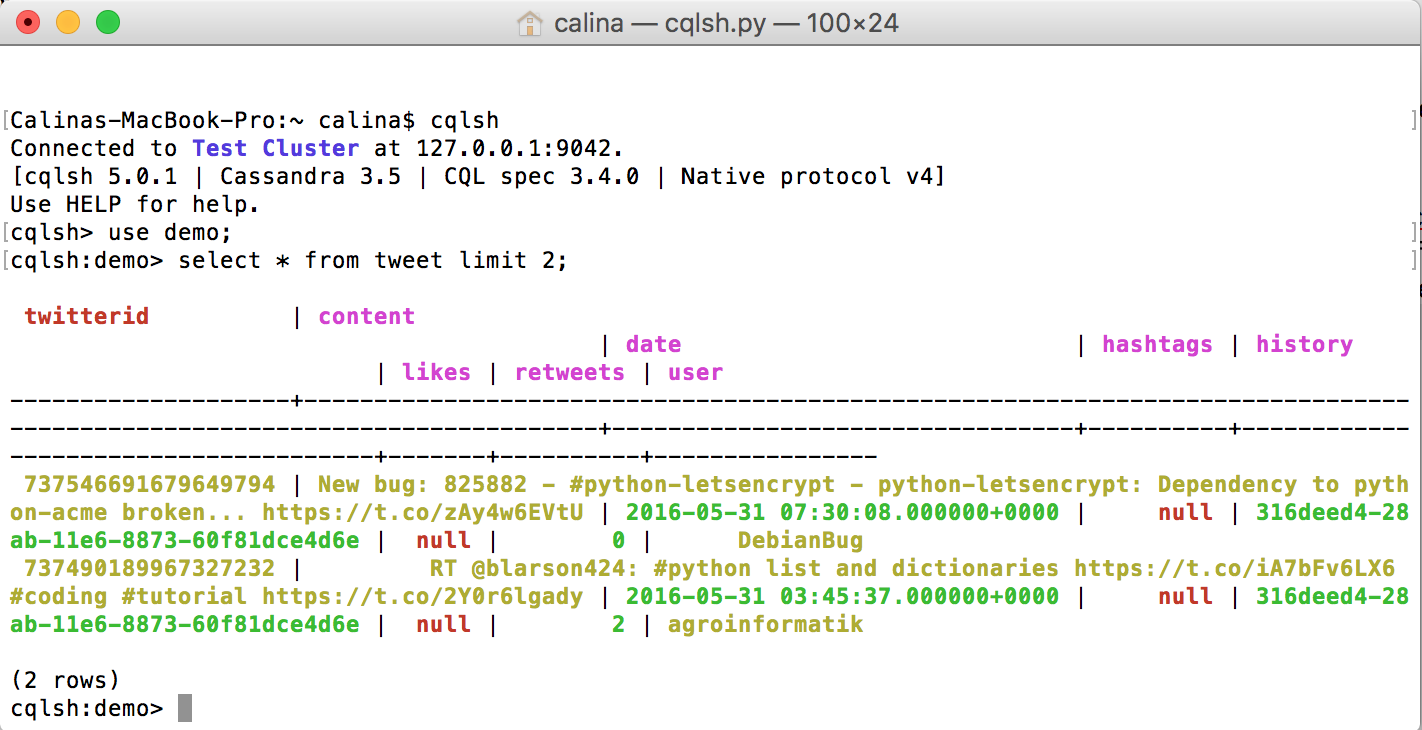
\includegraphics[width=0.8\columnwidth]{img/cqlsh.png}
    \caption{Demo of the cqlsh utility}
    \label{fig:cqlsh}
\end{figure}

The same functionality can be mirrored in Python using the following set of instructions:

\lstset{basicstyle=\scriptsize}
\begin{lstlisting}
from cassandra.cluster import Cluster

cluster = Cluster()
session = cluster.connect('demo')

 harvests = session.execute(
    """
    select * from tweets limit 2
    """
)
\end{lstlisting}

with the result being a generator which can be further consumed by the application. This means that it is easy to perform queries programatically, without much overhead, by employing the usage of this driver.

Cassandra queries are used throughout the application, both in synchronous and asynchronous application steps. Its speedy retrieval and updating of records is not a bottleneck, as API rate limits are.

\subsection{Database structure}
Two tables are used in our application. The \texttt{harvest} table containing columns:

\begin{itemize}
\item uuid (primary key, generated for each user-submitted harvest form)
\item start date (from which we harvest Tweets)
\item end date (up to which we harvest Tweets)
\item hashtag (used to query Twitter's API for statuses containing this particular hashtag)
\item done (boolean fag indicated whether the harvest has finished downloading Tweets)
\end{itemize}

The \texttt{tweet} table is used for storage of tweets belonging to histories and contains:

\begin{itemize}
\item twitterId (the id of that status on Twitter)
\item user (username of the author on Twitter)
\item content (textual content including hashtags)
\item date (of postage)
\item retweets (number of retweets, indicating popularity)
\item history (uuid of harvest that Tweet belongs to inside ATHENA)
\end{itemize}

\section{Harvesting tools}
The harvesting module as presented conceptually in \ref{fig:harvestpipe} was implemented in ATHENA using asynchronous job queueing. The user is presented with a form for submitting the harvesting job, consisting of a content field, start and end dates. An asynchronous job is launched via Python's Celery task library, which uses the tweepy library to connect to the Twitter Search API and Cassandra driver to save tweets and harvests.

\subsection{Celery for asynchronous jobs}
The Python library Celery\footnote{http://www.celeryproject.org} is designed for the fairly frequent development case where asynchronous jobs need to be managed. The Producer-Consumer architecture is implemented with Celery, as used in its real-time mode, while another option would be using Celery to run scheduled jobs. The job granularity in this case is indeed Harvest-level, with each job inside the Producer-Consumer queue is defined as the job of downloading one single, separate Harvest.

As previously stated, a huge advantage of Python is that third party libraries are highly compatible and easily configurable. Such is the case with Celery as well, setting up an asynchronous jobs taking very little effort:

\begin{enumerate}
\item install the \texttt{celery} library using \texttt{pip}
\item add configuration information to a celery.py file inside the application directory, including the task body and its decorator \texttt{@app.task(bind=True)}
\item import the function and use it. In the ATHENA Harvesting module context, the function was added as part of the Form validation customisation in Django's FormView class
\item install and configure a service broker such as Redis
\end{enumerate}

\subsection{Using Redis as a Celery broker}
Celery offers a variety of possible brokers for message transport through the job queue. Stable brokers are RabbitMQ and Redis, while others are in Experimental stages or offered by third parties\footnote{http://docs.celeryproject.org/en/latest/getting-started/brokers/}. Redis is an open source data structure store which can perform as a database or cache system, but in our case we are interested in its functionality as a message broker.

Installing Redis is straightforward using a downloaded package and even some available package managers such as Mac's \texttt{brew}. After the installation is complete, the Redis server can be fired up using the command \texttt{redis-server}. A splash screen with Redis' logo as ASCII art, such as the example in \ref{fig:redis} should appear, but connection to the running Redis server can also be tested by pinging:

\lstset{basicstyle=\small}
\begin{lstlisting}
$ redis-cli ping
PONG
\end{lstlisting}

\begin{figure}[ht]
    \centering
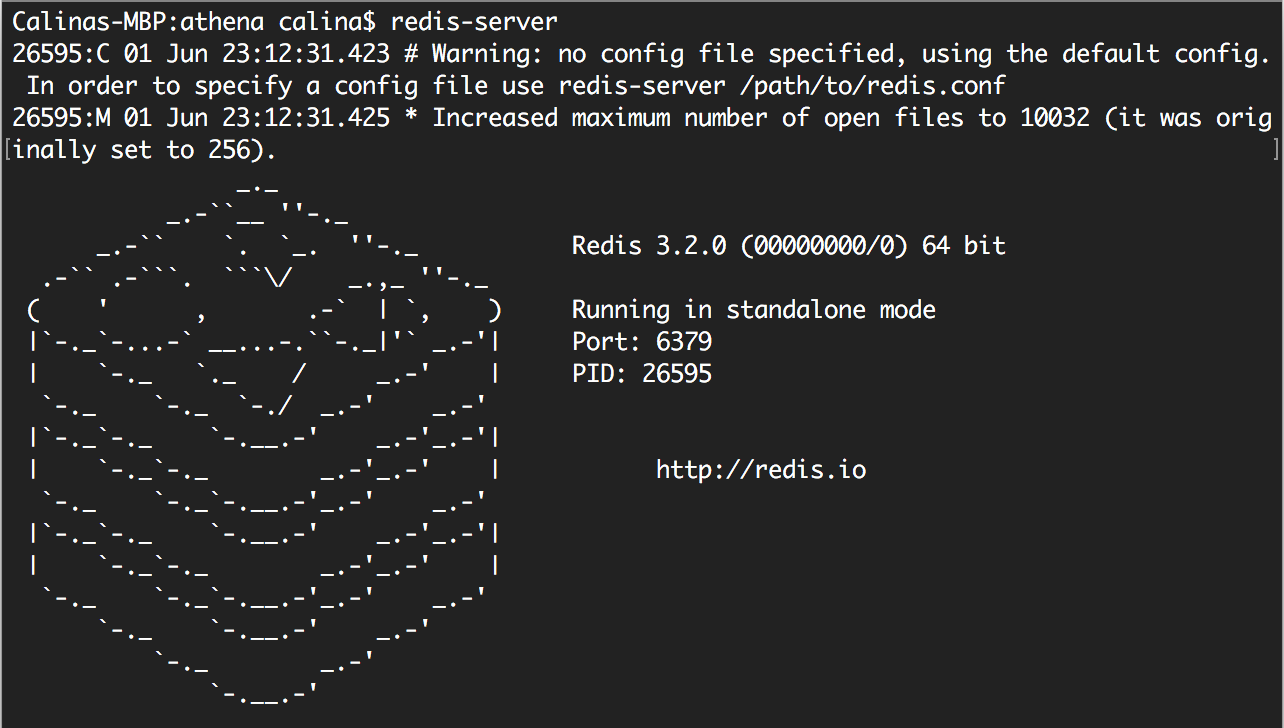
\includegraphics[width=0.8\columnwidth]{img/redis-splash.png}
    \caption{Redis splash screen}
    \label{fig:redis}
\end{figure}

After the Redis server is properly installed and running, there are some extra steps for hooking it up: adding the Redis configuration settings in our project's \texttt{settings.py} file and installing the \texttt{redis} library using pip. After all these steps are completed, running:

\lstset{basicstyle=\small}
\begin{lstlisting}
celery -A athena_app worker -l info
\end{lstlisting}

should confirm Celery's connection to Redis. Any tasks that were previously set up will now go through this job queue.

\subsection{Fetching data from Twitter using the Search API and Tweepy}
Once the general configuration of the asynchronous job is done, we can use the Twitter Search API to Harvest tweets per the specifications.

Twitter belongs to a series of web applications which fully understands the developers' need to hook into some of their features. Creating a Twitter application is easy from their developer support pages, with the creator receiving a set of OAuth access keys:

\begin{itemize}
\item a Consumer Key (API Key)
\item a Consumer Secret (API Secret)
\item an Access Token
\item an Access Token secret
\end{itemize}

For harvesting tweets, my approach uses a wrapper to Twitter's Search API called Tweepy\footnote{http://tweepy.readthedocs.io/en/v3.5.0/}. It is a library that handles connection and customised requests to the API, in a Pythonic fashion. Tweepy needs to be installed using pip, and then configured with the proper access keys (here in the code sample replaced with placeholders for security purposes):

\lstset{basicstyle=\small}
\begin{lstlisting}
from tweepy import OAuthHandler

consumer_key="XXXX"
consumer_secret="XXXXXXXX"

access_token="XXXX"
access_token_secret= "XXXXXXXX"

auth = OAuthHandler(consumer_key, consumer_secret)
auth.set_access_token(access_token, access_token_secret)
\end{lstlisting}

The way I am using this is by first setting up an \texttt{api} object which I will further query for statuses. I will initialise it using the \texttt{auth} object and a few flags:

\begin{itemize}
\item \texttt{wait\_on\_rate\_limit=True}. Flagging this indicates to the api object that whenever it reaches the API rate limits, it should not stop, but rather sleep for the required amount of time until new data can be acquired. This approach is preferable, since our harvesting takes place asynchronously and we do not mind the process sleeping for a while
\item \texttt{wait\_on\_rate\_limit\_notify=True}. Setting this flag tells the api object to print out a warning string to the console, indicating when it has reached the rate limit and at the beginning and end of the sleep cycle. E.g.:\lstset{basicstyle=\small}
\begin{lstlisting}
[2016-06-02 10:17:46,804: WARNING/Worker-2]
Rate limit reached. Sleeping for:
627
\end{lstlisting}
\end{itemize}

After setting up the API, a Tweepy Cursor class is used for querying it. This is initialised with the api object and parameters indicating the query we send to the server. This uses parameters defined by the user upon submitting the harvest form, refined by our application's specifications. The hashtag field is prefixed with a "\#" sign, start and end dates are formatted to "yyyy-mm-dd" and the language set to English, since extension to other languages is beyond the scope of this thesis.

The cursor will return a Pyhton generator, which means that the contents of the tweet list is rather consumed one by one, rather than having the whole list present at either point in time. Here, using Cassandra, we save the contents to the database.

\lstset{basicstyle=\small, breaklines=True}
\begin{lstlisting}
tweets = tweepy.Cursor(api.search, q='#' + hashtag, since=start_date, until=end_date, lang='en').items()

for tweet in tweets:
    session.execute(
     """
     insert into tweet (twitterId, user, content, date, retweets, history) values (%s, %s, %s, %s, %s, %s)
     """,
     (str(tweet.id), tweet.author.screen_name.encode('utf8'), tweet.text, tweet.created_at, tweet.retweet_count, key)
     )
\end{lstlisting}

The stored and completed harvests are now ready for the Enhancement step.

\section{Enhancement tools}
Enhancement tools are concentrated in the enhancement\_manager.py file/module where basic numerical calculations on the data is performed, alongside more complex transformations such as related hashtag collection and hashtag clustering. The process of enhancing data starts on the Enhancement tab, with the user being presented the list of available Harvests. The user decides on the harvest they want to enhance and display by clicking an icon next to the harvest's title.

\subsection{Simple numerical data}
A number of easily calculated, relevant data is calculated for the user and displayed on the enhancement results page. The number of tweets is calculated using a database query and displayed in a separate \texttt{<div>} on the results page.

\subsubsection{User-related data}
Upon consuming the tweet generator which resulted from the query, the data related to users is restructured as a Pyhton dictionary having the usernames of keys and the number of documents authored by those users, in the contex of the present harvest. The following numerical data is displayed related to users:

\begin{itemize}
\item the number of unique users contributing tweets to the enhanced harvest
\item the maximum number of tweets per user. The author's username is also presented in parantheses, and will usually represent a bot or a domain-related page, e.g. for the \texttt{\#pyhton} hashtag, the highest number of posts in a given day is posted by the user \texttt{@pyhtonbot\_}
\item the average number of posts per user, which is a metric indicating the general activity level of the harvest's generator hashtag
\end{itemize}

\subsubsection{Modeling the post numbers}
Since many a times the number of posts per user tends to skew towards pages and bots, it may be the case that the number of posts indicate a certain pattern. To analyse the eventuality of post numbers as an estimation of a power function, the \texttt{plfit} library was used. First the data was prepared as a list, from the users/posts dictionary described above. 

The \texttt{plfit} library was originally written in Matlab by Clauset et al \cite{clauset2009power} and later converted to R, Python and C++ modules by various developers. It handles calculations regarding data pattern fitting to a power law as described in \ref{plfittheory}. The library is suitable for non-domain-related data, being based on a combined maximum-likelihood fitting and goodness-of-fit tests. It was tested on twenty-four real-world data sets from unrelated fields of study and has found good results with power law fitting.

After importing the \texttt{plfit} library into the enhancement module, a plfit object is created. The tweet numbers are then fitted using the plfit method on the list described above. The minimum value and alpha are printed on the enhancement results page.

\subsection{Sci-kit learn}
Sci-kit Learn\footnote{http://scikit-learn.org/stable/} is proof of the fact that Python has recently gained much momentum in science and research. Its architecture is build on other stable and related Python science libraries, namely NumPy, SciPy and matplotlib. In fact, upon installation with the \texttt{pip} command line utility, sci-kit also installs these libraries as dependencies. According to a large number of scientists \cite{pedregosa2011scikit} and as displayed on their website, sci-kit learn is used for supervised and unsupervised data mining and data analysis endeavours, including:

\begin{itemize}
\item Classification
\item Regression
\item Clustering
\item Dimensionality reduction
\item Model selection
\item Preprocessing
\end{itemize}

Other important advantage of this library is its open souce BSD licensing. This means that, even tough it is a highly specialised tool, it is free to use for developers worldwide. The following presents \emph{sci-kit learn}'s employment in ATHENA.

\subsection{Related hashtag calculation}
Twitter uses a hashtag system to encourage users to tag data for proper search and visibility. Hashtags are words prefixed by a "\#" character, which represent categories of statuses. The hashtag system has been used on Twitter ever since its start, as opposed to other social networks such as Facebook, who only employed tagging much after being launched. Such other social networks have a hashtag disadvantage, since the system did not "catch on" with their users as naturally as it has on early-adopters such as Twitter.

On going into the realm of more complexly calculated data, as opposed to the numerical values extracted directly from the list of tweets, calculating a harvest's related hashtags is a more difficult task and is achieved using sci-kit learn. Figure \ref{fig:tweet} presents a sample tweet (the screenshot was taken on 7th June 2016), and it is clear empirically from such status messages that hashtags can be interpreted as category labels.

\begin{figure}[ht]
    \centering

\includegraphics[width=0.8\columnwidth]{img/tweet.png}
    \caption{Sample status message with hashtags}
    \label{fig:tweet}
\end{figure}

The tweet in Figure \ref{fig:tweet} also empirically demonstrates that the same post belongs to a number of related categories, in this case \emph{yoga}, \emph{fitness}, \emph{lolesport}, \emph{gym}, \emph{cardiotime}, \emph{sports}, \emph{workout} and \emph{zumba}. Indded these hashtags seem much related to one another, in this case, all belonging to a domain of sport and fitness.

Analysing each status' component hashtags will reveal related hashtags. As part of the enhancement process, we consider all the related collected tweets which compose a harvest and go trough the \texttt{get\_vocabulary} function, much like in the grammatical process of collecting a word's semantic field.

\subsubsection{Getting the hashtag vocabulary}
For the purpose of getting the list of related hashtags to our own harvest's base hashtag, we use a few customised components from the \emph{sci-kit learn} toolbelt. I start by vectorizing the list of tweets using the \texttt{TfidfVectorizer} with the following options:

\begin{itemize}
\item \texttt{min\_df=10}, to prevent hashtags who appear in less than 10 tweets appearing in our final list of results. This prevents noise generated by use-once hashtags through unusual, parody or disparate hashtags.
\item \texttt{max\_df=0.8}, to prevent flooding with most-common hashtags appearing in more than 80\% of the corpus
\item \texttt{sublinear\_tf=True} to use a sublinear function. A linear idf function may boost the document scores sometimes, but since the frequency of a term to relevance is usually a sublinear function, we use this option to ensure higher-precision results.
\item \texttt{use\_idf=True} to enable inverse-document-frequency re-weighting
\item \texttt{max\_features=25} to limit our search of most relevant related hashtags to a number of 25. We do this so that only the best most relevant hashtags are displayed for the user and prevent them being distracted by too much information.
\item \texttt{token\_pattern='\#[a-zA-Z0-9][a-zA-Z0-9]*'}. This option takes a regular expression (RegEx) argument which it uses to identify relevant tokens inside the corpus. Since we are only interested in hashtags and not other content words, the RegExp introduced forces the vectorizer to only consider "words" that start with a "\#' symbol and has one or more alphanumerical characters afterwards.
\end{itemize}

The sparse matrix indicating term frequency is obtained using the initialized vectorizer to \texttt{fit\_transform} the list of tweets' texts. Although a sparse matrix would overwhelm a non-expert user, and I have chosen not to display it as part of the enhancement results, the structure's content can be printed on the console and used for debugging and bird's eye correctness checking.

\begin{figure}[ht]
    \centering
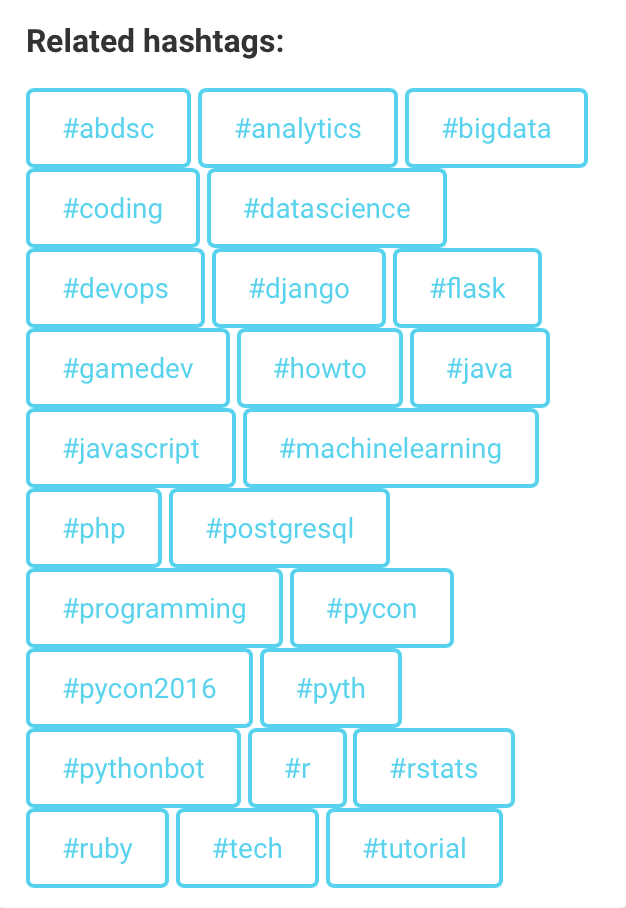
\includegraphics[width=0.4\columnwidth]{img/relhashtags.png}
    \caption{Example of related hashtags in a \#Python harvest over one day}
    \label{fig:relhashtags}
\end{figure}

We do however return the \texttt{vocabulary} variable. We calculate this by having the vectorizer perform the \texttt{get\_feature\_names()} method. This enables us to print a list of related hashtags on the enhancement results page in a separate \texttt{div}, as exemplified in Figure \ref{fig:relhashtags}. Indeed the empyrical data obtained in the example for the \#python hashtags showcases some of Python's most popular features (\#bigdata, \#machinelearning), tools (\#django, \#flask) and related technologies (\#javascript, \#ruby, \#r).

\subsection{Related hashtag clustering using KMeans}
Another interesting aspect the hashtags indicate is that there are some general directions (or common features) of our text. In a supervised approach, this could be tackled with an adnotated training dataset which would help classify the data. However, since ATHENA is based on user input and analysis of non-domain-related documents, such an approach is not appropriate.

One of the most classic approaches in classifying non-adnotated data is the K-Means clustering algorithm. Luckily \emph{Sci-kit learn} also contains tools for clustering approaches, including various implementations of K-Means variants.

Calculations start similarly to the approach described above, for related hashtags, but features an extra step for clustering. The concern for choosing a number of cluster centroids was similar to the one choosing the number of related hashtags to be displayed: A number of 5 centroids was chosen with the goal of having enough diversification, but not too many clusters to display, so as not to confuse the user. In a more domain-tweaked approach, the number of clusters would have been chosen according to the data's structure, but here it is a trade-off between the various factors explained.

A new \texttt{TfifVectorizer} object is instantiated with similar options, except for the \texttt{max\_df}, in order to also consider highly-used hashtags. After reproducing the \texttt{fit\_transform} step and obtraining the fitted set X, we apply the KMeans algorithm as such:

\lstset{basicstyle=\small, breaklines=True}
\begin{lstlisting}
from sklearn.cluster import KMeans
[...]

model = KMeans(n_clusters=true_k, init='k-means++', max_iter=100, n_init=1)
model.fit(X)
\end{lstlisting}

For the centroid initialisation, I chose the "K-Means++" algorithm described in \ref{kmeansplusplus}, a maximum number of iterations towards the solution of 100. The \texttt{n\_init} option instructs the K-Means algorithm to run  just once with different centroid seeds. In case a larger number would have been chosen, the output of the algorithm would have been the best output during these runs.

\subsubsection{Ordering and displaying the hashtag clusters}
The main issue with clustering generation, as directly resulted from the \emph{Sci-kit} K-Means algorithm, is that the clusters are not ordered. Items are assigned with some probability to each cluster, but there is no clear representation and collection of those clusters. In order to properly display these clusters on the results page, though, they need to be sorted and formatted.

\lstset{basicstyle=\small, breaklines=True}
\begin{lstlisting}
order_centroids = model.cluster_centers_.argsort()[:, ::-1]
terms = vectorizer.get_feature_names()
clusters = {}

for i in range(true_k):
    cluster_name = 'Cluster ' + str(i+1) + ':'
    cluster = {}
    for ind in order_centroids[i, :10]:
        cluster[ind] = str(terms[ind])
    clusters[cluster_name] = cluster

    return clusters
\end{lstlisting}

Note the similarity to the previously described feature. The terms are fetched just the same, and then their assignment to the clusters is checked. The resulting structure is a dictionary consisting of cluster names as keys and hashtags (from the same cluster) as values.

They are returned to the controller, then to the front-end part and displayed via Django's templating engine. For a better understanding of their separation, each cluster is placed into its own div with Bootstrap's \texttt{well} CSS class, which adds a separate wrapper and colouring to its contents. Figure \ref{fig:clusters} presents an example of such a clustering.

\begin{figure}[ht]
    \centering
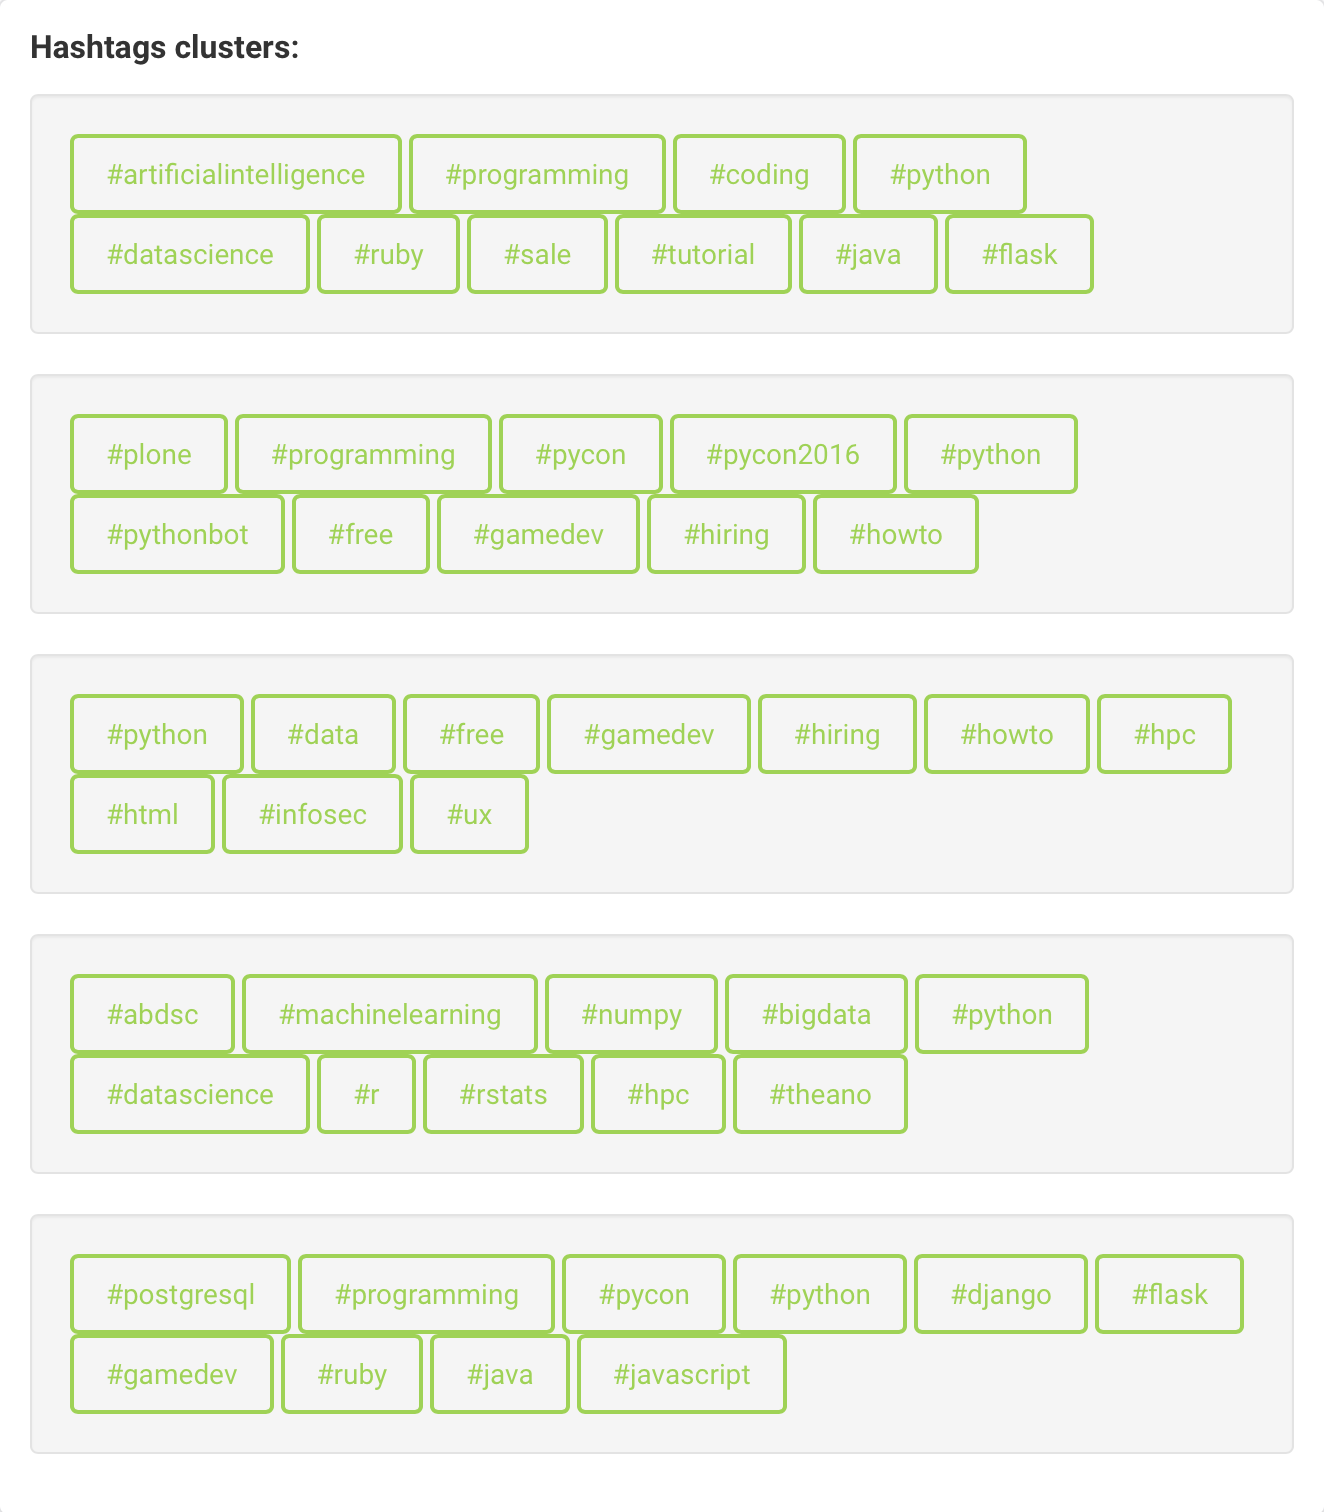
\includegraphics[width=0.7\columnwidth]{img/clusters.png}
    \caption{Example of clustered hashtags in a \#Python harvest over one day}
    \label{fig:clusters}
\end{figure}

It can be seen in the example that the clusters follow a structure similar to Python's main fields of development.

\begin{enumerate}
\item the first cluster is correspondent to some genric Python fields: \#flask, \#coding, \#artificialintelligence
\item the second cluster is correspondent to Python conventions, promotions and opportunities for development: \#free, \#gamedev, \#hiring, \#pycon
\item the third cluster relates to front-end technologies and their prevalence in Python conventions: \#html, \#ux
\item the fourth cluster relates to Python's endeavours in machine learning: \#machinelearning, \#bigdata, \#numpy, \#datascience, \#r, \#rstats
\item the fifth cluster is a collection of technologies related to Python or generally used alognside it: \#postgresql, \#django, \#flask, \#javascript
\end{enumerate}

New clustering is calculated with every refresh, and the user can observe a high degree of convergence for rich hashtags such as our \#python example. For one-fold or loosely related hashtags, the number of centroids chosen might indeed be too large.

\section{Normalisation}
\subsection{Reasons and options}
As previously discussed, many a times the dataset is skewed due to spikes and outliers such as pages and bots. The normalisation step helps with the process of eliminating outliers and possible fakers, by flattening the dataset to a single representative post per each user. This is done mostly because professional pages intentionally use repetitive hashtags to promote certain events. On the other hand, bots scan for and retweet statuses which feature specific content, which results in the flooding of the dataset with promotional messages. Both these series of events lead to skewed dataset wich is easily recognisable by its fitting to a power function.

Remember that the Enhancement step only takes regular harvests as inputs, as it calculates power set fitting, likely pages and outliers etc. In a similar fashion, the Analysis step will only consider normalised harvests as permitted input. This means that output of the Normalisation step should be properly stored, in a separate table.

It must also be noted that the Normalisation step is still in its early proof of concept ages, since the main focus of this application was to develop and validate the Harvesting, Enhancement and Analysis steps, and only then add more functionality to the Normalisation module. Proper Normalisation should indeed take into consideration various factors:

\begin{itemize}
\item flattening process: 
\begin{itemize}
\item one post per user, to remove outliers such as pages and bots
\item multiple posts-only, to analyse only regular users, which use the hashtag more times, which would filter out accidental ones with opinions that might be unrepresentative for the community
\item popular posts-only, considering only posts with retweet count larger than a threshold $r$
\item liked posts-only, considering only posts with like count larger than a threshold $l$.
\item combinations of the above options
\end{itemize}
\item time period considered
\begin{itemize}
\item short term options: $n$-days with $n\leq7$, $m$-hour normalisation
\item long term options: $n$-days with $n>7$, which would also imply the possibility of streaming harvests on a longer period, per Twitter API's rate limits.
\end{itemize} 
\end{itemize}

Each normalisation method has its very own advantages and drawbacks, so in order to choose a viable normalisation method to implement, the following was considered: Unfortunately with promotional messages such as those posted by pages and bots, the retweet and like counts is often tied to some form of prize or gratification a user gets for sharing the content. This means that the popularity of the tweet is many a times artificially boasted using a variety of marketing methods. Also, it might be the case that few users actually post multiple tweets in a short-term amount of time, which rules out the second option of flattening as well.

Current implementation restricts normalisation options to one post per user and one-day date limits. However, the code is designed in such a fashion that new options should be added easily, when the need arises.

\subsection{One post per user, one-day limit normalisation process}
The process I describe below is currently the only allowed Normalisation process, with more to come after testing and user validation of the ATHENA proof of concept app. This method of normalisation intends to remove outlier influence of pages, bots and fake accounts.

The first interface presented to the user in the Normalisation step is a form containing the list of harvests in a dropdown. After submitting the form, the selected harvest is sent to the \texttt{normalisation\_manager.py} file through the controller. This manager file contains the process necessary to fetch the harvest's tweets from the database and flattening the result into a list.

The method used was the classical approach of duplicate removal using HashMaps (as implemented in the Python dictionary data type). Using the username as the dictionary's key, the last occurrence in the list of tweets for each user is considered. The value of this result dictionary is a tuple of tweet id and tweet content, which are later used in the Analysis module. Of course, the tweet's post date is also considered, in order to filter out tweets outside the date limit.

Results are stored in the \texttt{normal} database table, which has a structure consisting of the following columns:
\begin{itemize}
\item original harvest uuid, which facilitates comparison between corresponding normalised and regular harvests
\item name of the normalised harvest (formed using the original harvest's name and the normalisation type details)
\item JSON-serialised normalised dictionary resulting from the normalisation step
\end{itemize}

Or, as CQL script:
\begin{lstlisting}
CREATE TABLE normal (uuid uuid, name text, content text, PRIMARY KEY(uuid));
\end{lstlisting}

Multiple formats would have been suitable for serialisation if persistence only was considered. But in the idea of adding a RESTful module to the application, enabling its use from mobile and web applications seamlessly, the normalisation result is stored in a JSON format. JSON is a widely-spread and widely-used format for REST service communication and is easily integrated with Python and Django via the \texttt{json} library. The contents of the Python data structure is encoded using \texttt{json.dumps()}, while the loading from a string and into a Python data structure can be achieved using \texttt{json.loads()}.

\section{Analysis}
The Analysis module features a lot of similarity to both Enhancement and Normalisation, except that in both cases, the pages contain double the harvests. Firstly, the form step of Analysis contains two dropdowns which are populated with normalised harvests. After choosing a pair of harvests for comparison, the application redirects to a page displaying the analysis results.

As per previous modules, this one also has a dedicated manager file, called \texttt{analysis\_manager}. Analysis jobs are therefore passed from the controller to the manager and the results are sent back after calculation. A number of analysis types are run on the normalised harvests, including common vocabulary, common users and post proportions.

\subsection{Retrieving the normalised results}
The task of retrieving the previously saved normalised results is a fairly simple one, consisting of connecting to the database, running a query to select the two normalised entries as selected in the form (using their respective uuids) and deserialising the JSON string in the content using the \texttt{json.loads()} function. The deserialised result is exactly as the one calculated in the Normalisation step, i.e. the keys are the users and the values are tuples of significant data, including tweet content.

\subsection{Calculating the common vocabulary}
The common vocabulary of hashtags is a type of analysis inspired from the previous Enhancement step. We are interested, in case of hashtag pairs belonging to the same fields or domains, in their very own, particular characteristics (handled here with Enhancement), but also in some common values which the share. One such important question is whether there are any common labels between the two.

Common vocabulary generation is very much similar to vocabulary generation, as done in the Enhancement module. Hence the calculation consists of both respective vocabularies intersected. This means that the vocabulary function from enhancement can be reused in a DRY (Do not Repeat Yourself) fashion. The operation of intersection is done using the \& operator between the two sets, which is an efficient way of getting the result without much code written.

Figure \ref{fig:commonvocab} shows an example of results for the comparison between one-day normalisations of the \#python and \#php hashtags, indicating two general categories the two belong to (\#programming and \#coding), and two technologies usually associated to them, one on the front-end side (\#javascript) and one on back-end (\#java)

\begin{figure}
    \centering
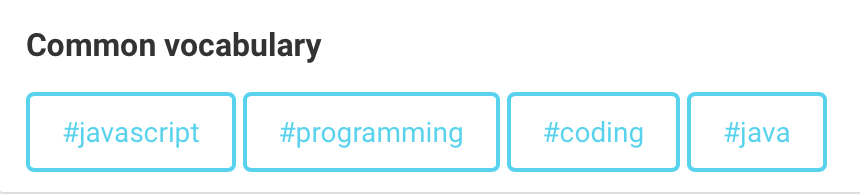
\includegraphics[width=0.5\columnwidth]{img/commonvocab.png}
    \caption{Example of common vocabulary in \#Python vs \#PHP comparison}
    \label{fig:commonvocab}
\end{figure}

\subsection{Calculating common users}
Common users are calculated in a similar fashion to that described above. Since the result deserialised from the database is a dictionary with unique keys (Python dictionaries are based on an underlying HashMap structure), the only task is to combine the two key arrays using an intersection operator, as previously done for the vocabulary part, e.g.:

\[common\_users = set(h1\_users) \& set(h2\_users)\]

\subsection{Calculating post numbers and proportions}
Another important metric is the prevalence of posts belonging to a harvest as part of the domain. In comparing two normalised harvests, we are interested in the proportion of each exclusive tag and also the number of common posts. These metrics show whether one or the other hashtag is the most productive in number of posts, which may indicate number of supporters. Furthermore, by analysing the numbers and proportions of these posts, we can deduce whether the domain is clearly split between the two hashtags, or whether there is a lot of gray area, which contains posts belonging to both categories. This latter option would indicate that supporters of both concepts are fluid and have no clear preference, while a clear separation could indicate die-hard fans.

Of course this relation can be exploited in a number of ways. In a very hostile, polarised domain, the user can analyse the risks of appealing to one of the groups, while rejecting the other. However in a cohesive domain with much middle ground, a good option is to appeal to the general unifying concepts.

In order to calculate the domain breakdown between the two normalised harvests, we consider users as a point of reference. We have already calculated the set of common users during the previous steps, so now we calculate the difference sets using the lists of posting users in each harvest and excluding the common ones.

Of course displaying the raw numbers on the results page doesn't help the user that much. It is therefore necessary to perform some extra steps to indicate the polarisation of the domain between the two hashtags: displaying the numbers as a graphical pie chart. Such a chart indicates the proportions of users who post exclusively for each hashtag and common users, who represent the middle ground.

Figure \ref{fig:piechart} presents the results for the user proportions between two hashtags: \#python and \#php. The results indeed seem to match with empyrical real-life data, since the two are both back-end programming languages and it is rarely seen that both are used by the same people or in the same projects. Results also display a highly-polarised domain, with a slight better cult of Python, which can be confirmed from other sources such as the TIOBE index, which maintains Python is more popular than PHP.

\subsubsection{Displaying the chart using Google Charts API}
A number of approaches for HTML charting are available for free use. Some work primarily on the back-end with image generation, while some are exclusively front-end. Among the simplest and easiest to use approaches is using Google Chart API, a javascript library for front-end chart generation. The image in \ref{fig:piechart} is captured from the application and is indeed generated using Google Chart API. The code is fairly straightforward, using javascript on the front-end side, from the list of values.

\begin{lstlisting}
var data = google.visualization.arrayToDataTable([
      ['Norm. Harvest', 'Number of posts'],
      ["{{ h1 }}",     {{ proportions.0 }}],
      ["{{ h2 }}",     {{ proportions.1 }}],
      ["common",     {{ proportions.2 }}],
    ]);
\end{lstlisting}

Note that the curly brackets used are from Django's templating engine, and are variables which are passed from the controller onto the view. When executing the javascript code, the values are already replaced with the corresponding values and will execute like normal strings or numbers within the code.

Hovering the mouse over one pie chart slice generates a dialog containing both the raw number and the proportion from the total, as shown in the figure as well, onto \emph{php one day normalisation}.

\begin{figure}
    \centering
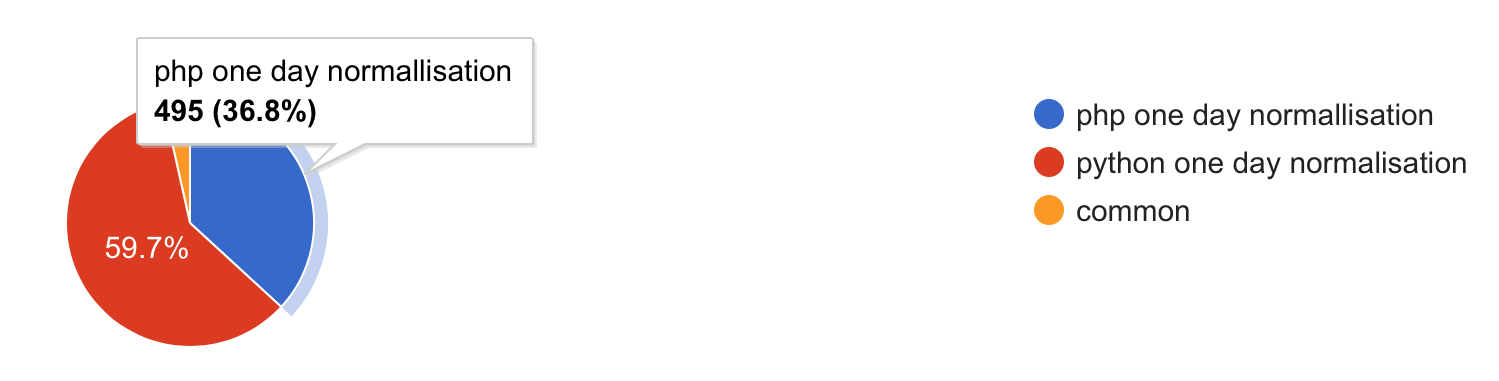
\includegraphics[width=\columnwidth]{img/piechart.png}
    \caption{Proportions of users who post \#Python vs \#PHP tagged statuses}
    \label{fig:piechart}
\end{figure}

\section{Code organisation}
Generally speaking, the code is organised in a classical MVC (Model-View-Controller) fashion, with specifics related to Django's recommentations. As per their recommended usage, the functionality is separated into an app called \texttt{athena\_app} found in the \texttt{athena} workspace, under a virtual environment wrapper with Django 1.8 installed. 

\subsection{File and folder structure}
As Django tends to encourage reusability, some of the scaffolding and file structure is generated via commands using the \texttt{manage.py} command line utility. E.g., upon creating a new app, a directory structure is also created containing:

\begin{itemize}
\item \texttt{urls.py}, the file which contains URL path definitions and directs received data to the corresponding views, as defined by the user. Our application currently defines a total of 8 URLs, for the index page, harvest, enhancement, normalisation and analysis page as well as some result pages. The local \texttt{urls.py} file is imported into the main \texttt{urls.py} which resides in the root of the project.
\item \texttt{views.py}, the file which contains what other frameworks call "controller actions". These functions determine the behaviour of the application when encountering the data matched by respective entries in \texttt{urls.py}. As a general best practice, our functions in \texttt{views.py} either inherit and override significant parts of Django generic views\footnote{Code templates for widely-used functionalites such as CRUD, forms or simple HTML rendering views}, or use minimal code and delegate to manager files for the core functionality.
\item \texttt{models.py}, which should contain model definition. This file was not used, since database queries were written manually in CQL, which is not that well supported by Django's migration creating structure for models and migrations.
\item \texttt{forms.py} which contains form definitions, holding part of the functionality, field definitions and validation instructions
\item other various folders such as the \texttt{static} folder where static files such as images, CSS and JS are stored, and the \texttt{templates} folder where html views are stored. Our application's static folder contains various Twitter Bootstrap CSS and JS elements for beautifying the front-end, while our templates directory holds a number of 6 individual views (mostly corresponding to the URLs enumerated above) and one \texttt{base.html} view which the others use as a general template. This enables us to only overwrite those sections which change and leave the menu and headers generally intact.
\item some other files and folders which we have not used and are beyond the scope of our application, such as \texttt{admin.py} (which should define administrative actions with Django Admin) and others.
\end{itemize}

Python's import structure is defined using file names and classes/functions defined inside those files. This makes it easy to use functions from files such as managers, by simply importing those functions. The separation of concerns principle is very important for proper maintenance and good functionality of the code, so the controllers stay light and handle Request processing and Response sending, while the core work is done separately in managers. The application defines a number of four managers:

\begin{itemize}
\item \texttt{harvest\_manager.py}, dealing with harvesting jobs and used primarily from the harvest parts of the \texttt{view.py} file
\item \texttt{enhancement\_manager.py}, dealing with the enhancement-concerned parts of the application
\item \texttt{normalisation\_manager.py}, dealing with flattening the datasets as instructed by the corresponding actions in \texttt{views.py}
\item \texttt{analysis\_manager.py}, containing analysis functions and used by the Analysis module
\end{itemize}

As previously stated, Python's simple structure make it easy to import functions from the managers inside the views using specific commands and then straightforwardly using the function, e.g.:

\begin{lstlisting}
from athena_app.harvest_manager import get_harvests
[...]
result = get_harvests()
\end{lstlisting}

\subsection{Using Django generic views}
Django offers the possibility of reusing specific classes from their very own codebase, classes which were designed for repetitive tasks. As opposed to having programmers code their very own implementations of rendering simple HTML views, creating and validation forms or performing CRUD (Create, Update, Delete) funcionalities, these classes, called generic views, can be directly used, or efficiently customised by overwriting a few attributes or methods.

ATHENA uses Django's \texttt{FormView} and the basic \texttt{View}, imported from

\texttt{django.views.generic.edit} and 

\texttt{django.views.generic.base}

respectively. The former is used for creating the Enhancement and Normalisation harvest selection page, and the Analysis pairwise normalised harvest selection page. FormView is also used when creating the harvest and is perhaps the most representative example, combining fields of various types and a special success method performed on return.

The HarvestForm is defined in \texttt{forms.py} and used inside the FormView in \texttt{views.py}. Inside the class definition an extra method was added, called \texttt{create\_harvest}, which is not an override of any parent method, but instead contains instructions on performing the asynchronous job of creating the harvest. Otherwise, the rest of the Form definition consists of field declarations with their corresponding types:

\begin{itemize}
\item \texttt{hashtag} as type \texttt{CharField}, the hashtag used for searching tweets on Twitter API
\item \texttt{start\_date} as type \texttt{DateField}, the beginning date for filtering tweets
\item \texttt{end\_date} similarly, represents the end date for tweet filtering
\end{itemize}

HarvestView inherits from Django's FormView and overwrites some fields and methods, which are somewhat instructive for understanding the other customised Forms and FormViews defined inside the application's codebase:

\begin{itemize}
\item template name: path of the HTML template to render
\item form class: the HarvestForm we defined in \texttt{forms.py} and imported here
\item success url: where the view should redirect upon form submission and success
\item get context data(): defines extra variables to be passed to the templating engine. In our case, it is the list of available harvests.
\item form valid(): extra validation and/or steps to be performed in case of success
\end{itemize}

In regards of the classic \texttt{View} generic, its only overwritten method was \texttt{get()} which instructs the view on the course it should consider when receiving a GET-type HTML request.

\subsection{List comprehensions and other Python specifics}
Python is a language of simplicity, but it is also a language difficult to understand from the outside. Its focus on simplicity starts from the building blocks: no visibility modifiers, easy import management, indentation-based execution blocks. However, some simplifications may seem obscure.

One of such shorthand becoming cipher is the declaration of arrays and lists, as in:
\begin{lstlisting}
    tweet_texts = []
    tweet_users = {}
\end{lstlisting}

This snippet first declares an array called tweet\_texts, while the second, tweet\_users, is a dictionary. To complicate things even worse, tuples are declared using round braces. This is in opposition to the generally verbose approach of other programming languages and is important to note.

On a related note, list and dictionary comprehensions are an efficient way of creating or filtering a list or dictionary with as less code written as possible. Code such as:

\begin{lstlisting}
[ ( x.uuid, x.name) for x in all_harvests ]
\end{lstlisting}

may be perceived as ambiguous for unfamiliar users. However for Python developers it becomes clear that this snippet produces a list of tuples from the iterable \texttt{all\_harvests}, with tuples containing the iterable element's uuid and name. In English, what this does it that it filters out some unnecessary properties in all harvests and transforms the list of objects into a simple list of pairs(uuid, name).

\subsection*{Summary}
In this section the details of implementation inside ATHENA were explained. The choice of Python and Django as programming language and frameowrk respectively were motivated by their large-scale use in developing scientific applications and web applications in general. The list of third party libraries was covered, with focus on particular libraries and their usage throughout the application.

The persistence model was chosen to be non-relational and scalable, in order to support scaling the system to a larger number of nodes and eventually moving towards a distributed web application. The task of fetching Twitter statuses was handled using asynchronous job running, using the Producer-Consumer architecture, via the Celery library with Redis as a message broker. This approach ensures the user doesn't have to wait for a job to finish before continuing to use the application independently. Inside the job, rate limits and concrete Twitter API communication were handled using Tweepy, a Python wrapper. The resulting, grouped information is called a Harvest.

The Enhancement step displays numerical data, a harvest's related hashtags and uses the acclaimed Sci-kit library to perform clustering on domain hashtags, using the K-Means algorithm. Another issue ATHENA tackles is the fitting of the post numbers dataset to a power function, investigating on outliers such as pages, bots and fake accounts producing significally more content than regular users.

The Normalisation step flattens the data set in a "one post per user, one day" fashion, with other normalisation options currently in development. The Analysis step uses the data flattened, filtered and stored by Normalisation to run a comparison between two harvests. Such data includes vocabulary commonalities and polarisation analysis.

The final part of this section approaches Python particularities which are used in the application but might seem unfamiliar to developers coming from different backgrounds, such as Java or PHP, where coding is usually more verbose.